\section{AndroFleet: a large-scale emulation platform}

\begin{frame}{Simulation vs. Emulation}
    \metroset{block=fill}
    \begin{block}{Simulation}
        A simulator sets up a similar environment to the original device's OS, but doesn't attempt to simulate the real device's hardware. 
        Some programs may run a little differently, and it may require other changes (like that the program be compiled for the computer's CPU instead of the device's).
    \end{block}
    \begin{alertblock}{Emulation}
        An emulator works by duplicating every aspect of the original device's behavior. 
        It basically simulates all of the hardware the real device uses, allowing the exact same software to run on it unmodified.
    \end{alertblock}
    \tiny{\url{https://www.quora.com/What-are-the-differences-between-simulation-and-emulation}}
\end{frame}

\begin{frame}{AndroFleet}
    \begin{itemize}
        \item Based on Docker
        \item Easily deployable
        \item All in a single container
        \item GPS scenario runner
    \end{itemize}
\end{frame}

\begin{frame}{AndroFleet Architecture}
    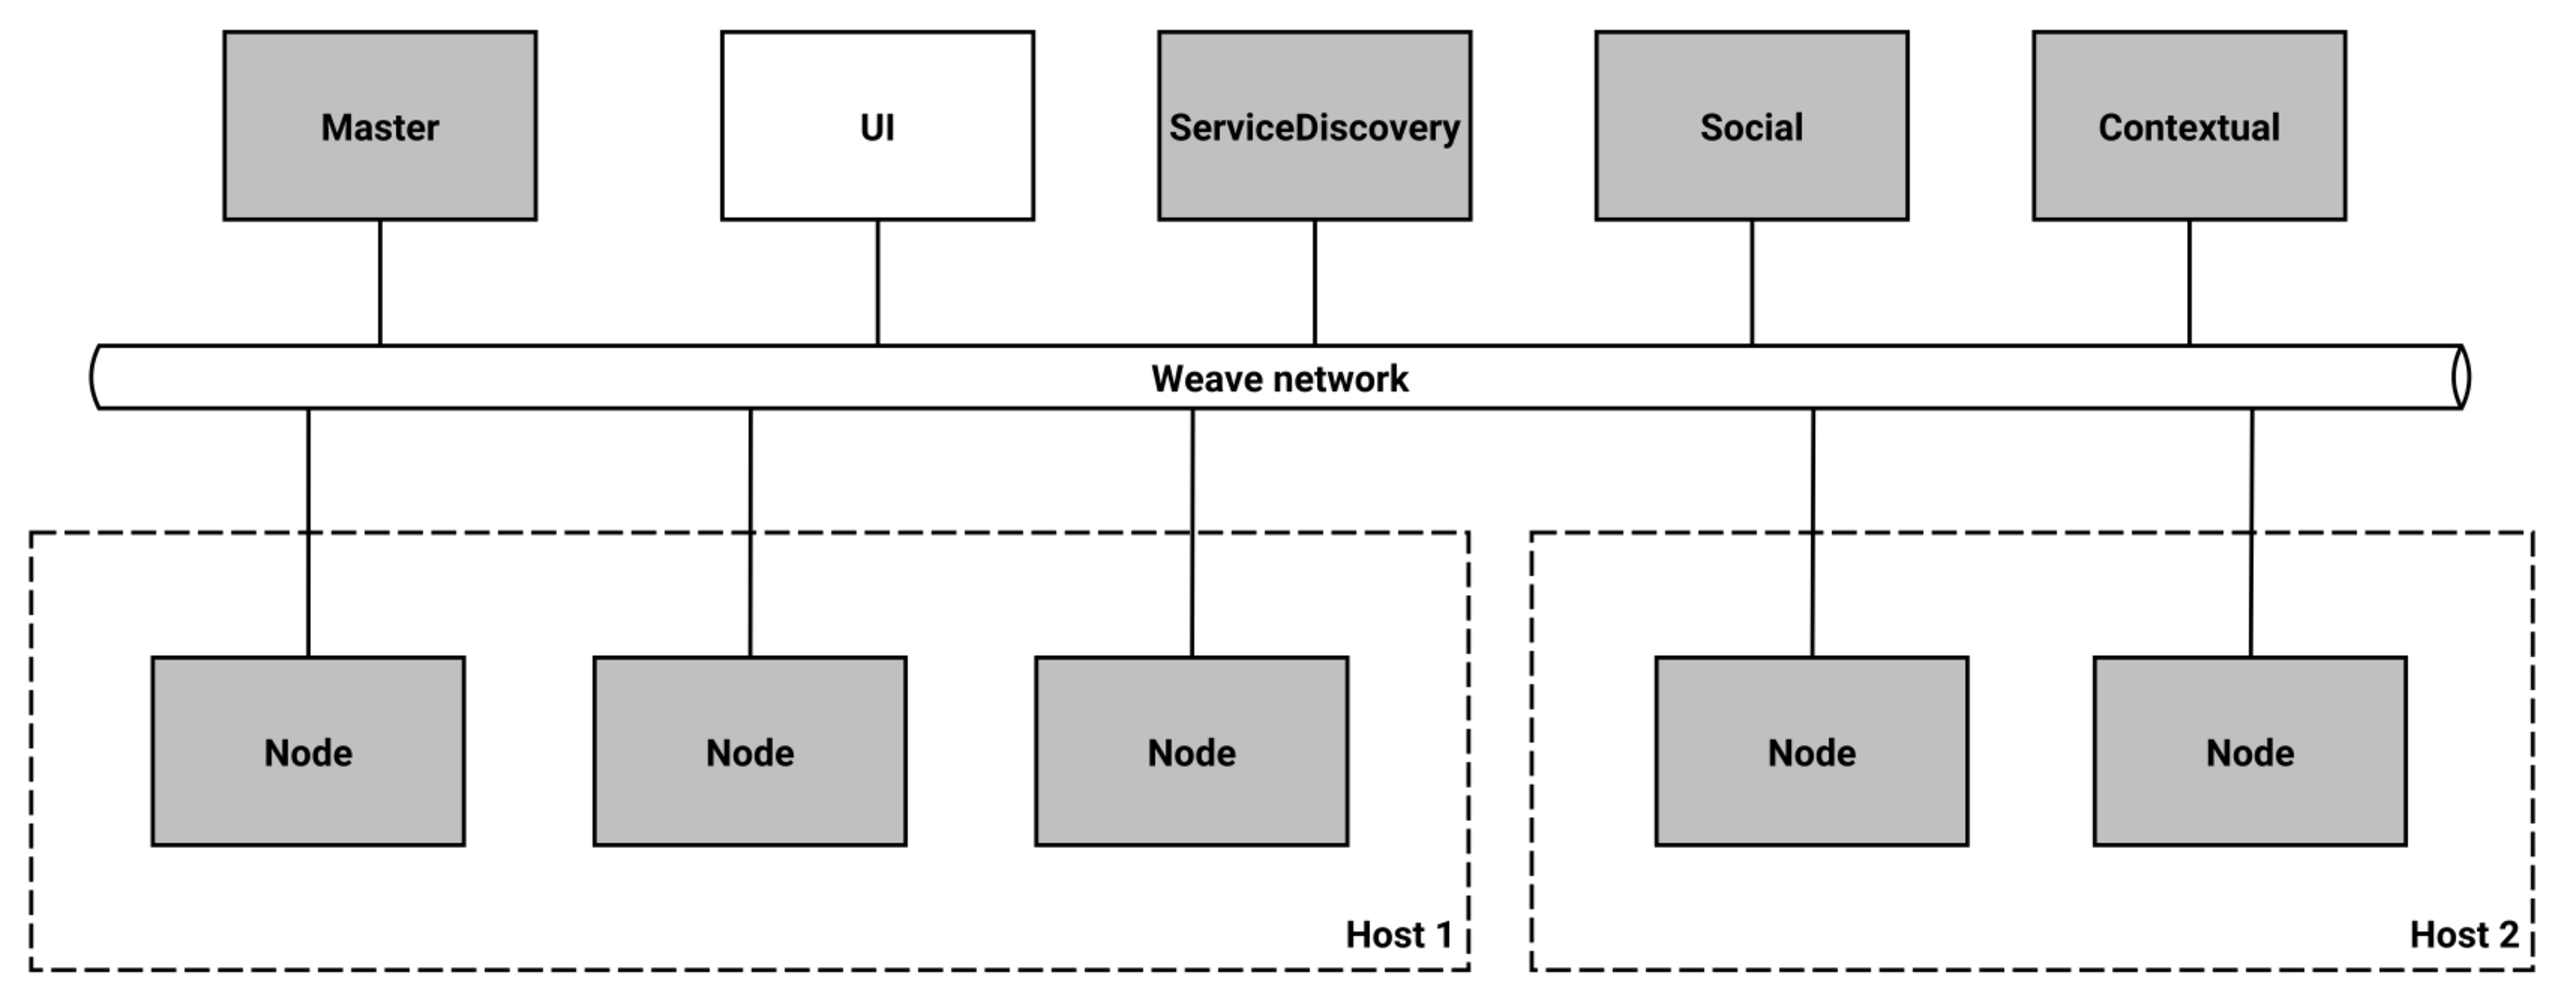
\includegraphics[width=\textwidth]{figures/androfleet}
\end{frame}

\begin{frame}{Wi-Fi Direct simulation}
    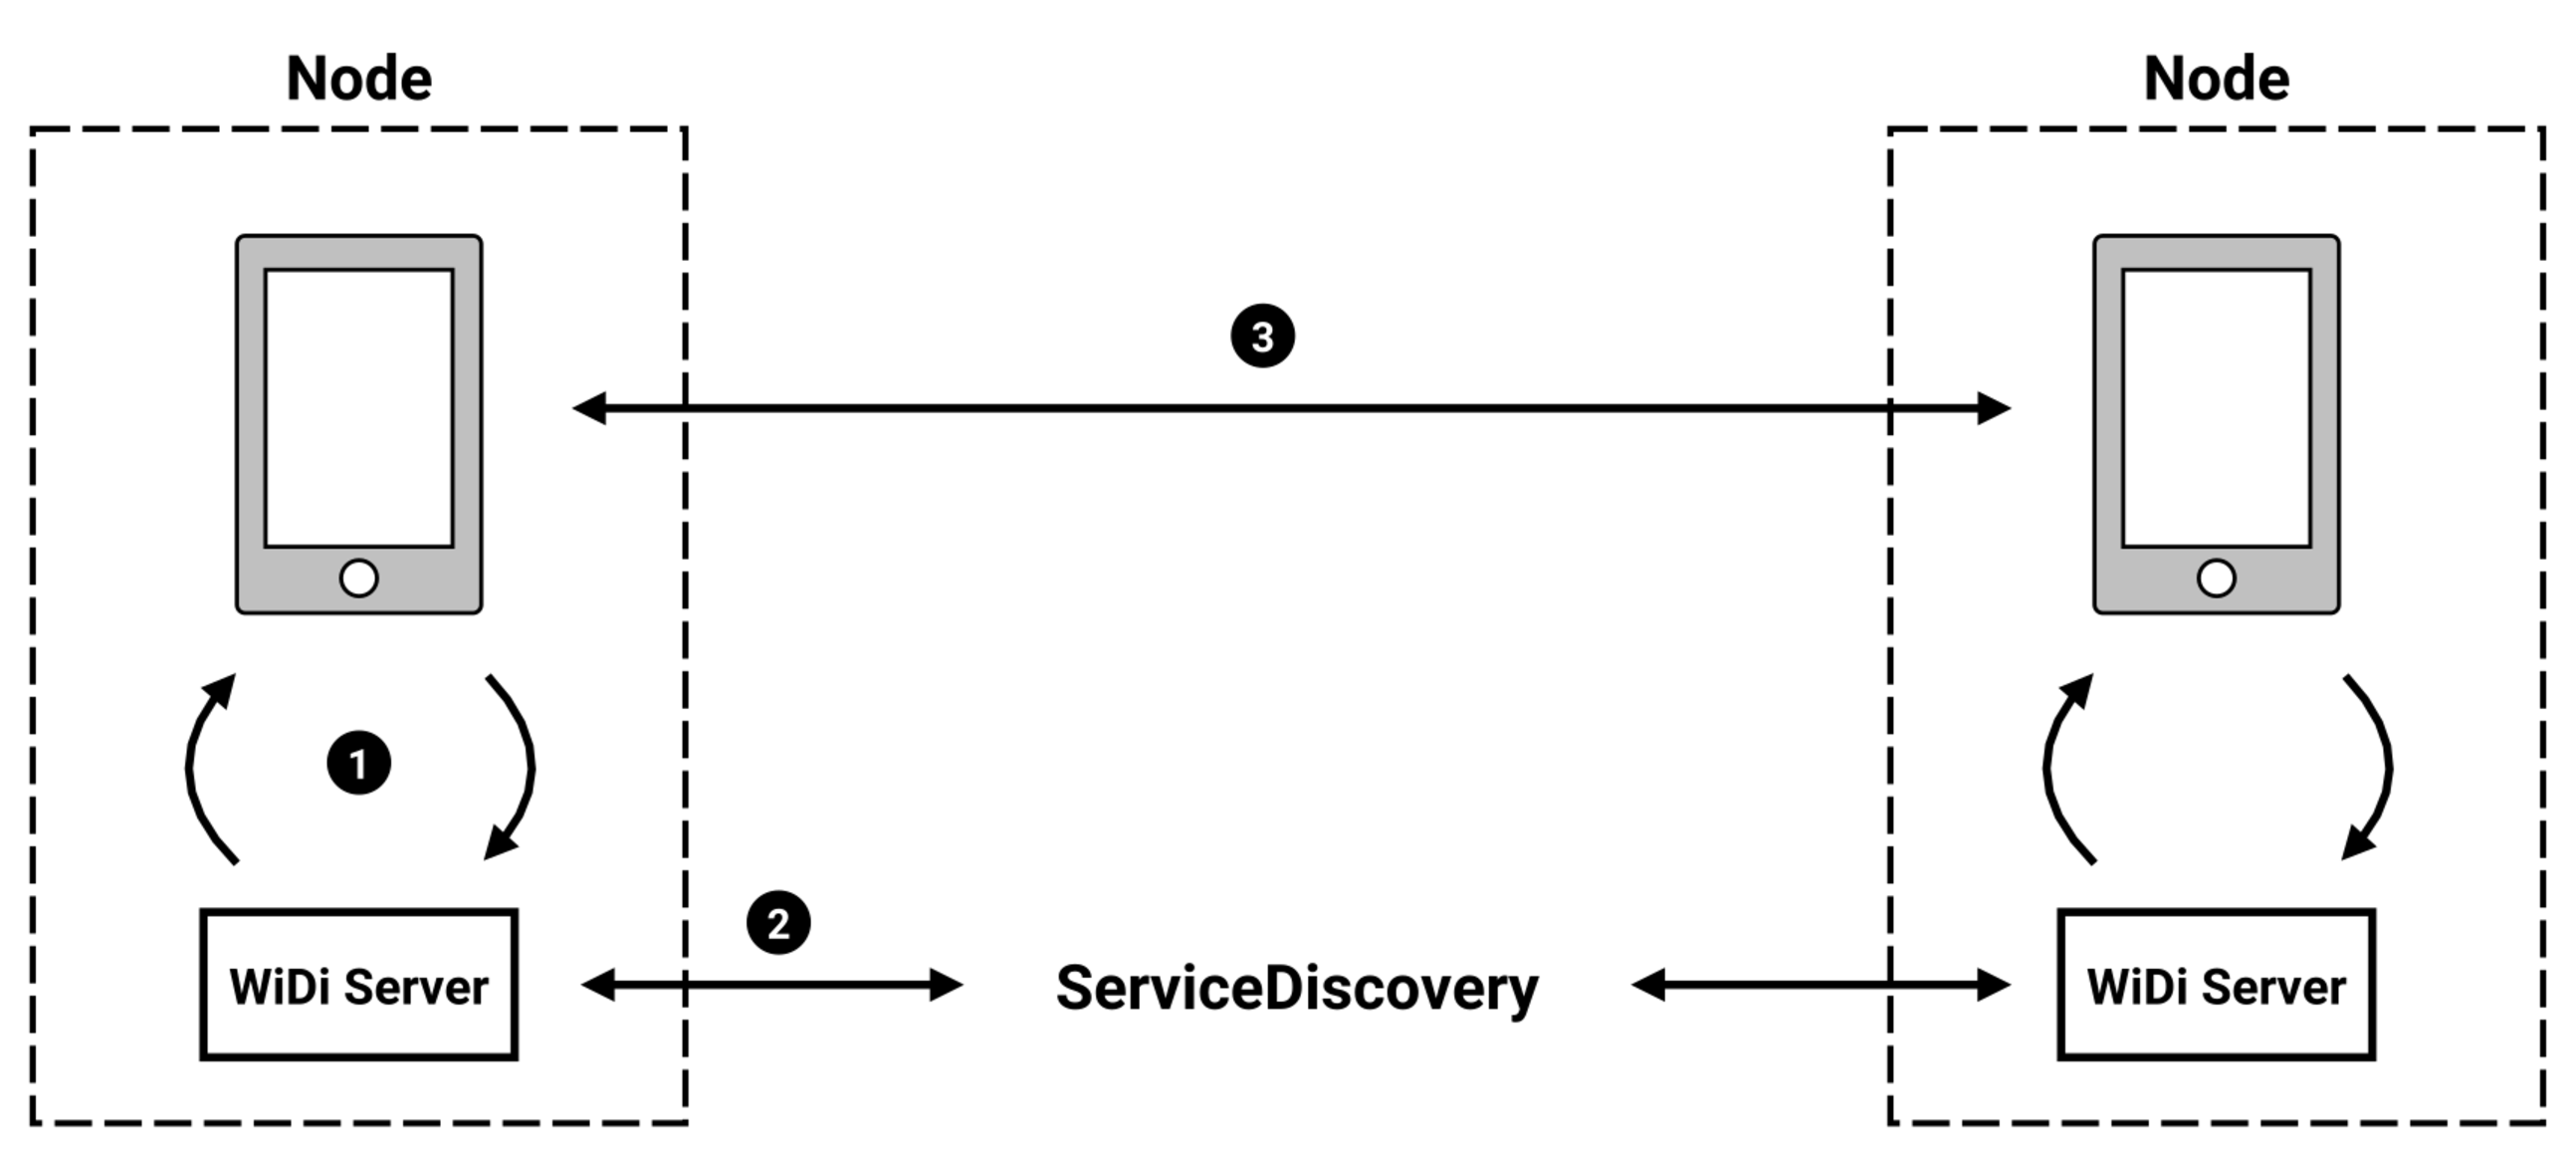
\includegraphics[width=\textwidth]{figures/widi}
\end{frame}

